\chapter{画像情報の処理}
\section{\purpose}
\matlab を用いて,画像に対して,カラーチャネルの操作,量子化数変換,階調反転,閾値処理,画素値に対するヒストグラムを作成する.
この実験では,上記の画像処理と合わせて,画像の肌色抽出と,微分フィルタや平滑化フィルタなどのフィルタの適用や色空間変換,肌色領域を抽出する.
さらに,画像を2次元フーリエ変換し,パワースペクトルを出力する.出力したパワースペクトルに対して,周波数フィルタを適用し,結果を考察する.
\paragraph{\kadaiaa}RGB色空間の画像を,緑チャネルだけを抜き出してグレイスケール画像を作成する.赤チャネル,青チャネルについても同様にグレイスケール画像を生成する.さらに,RGB画像の赤チャネルと青チャネルを入れ替えたカラー画像を作成する.
\paragraph{\kadaiab}グレイスケール画像を生成する.緑チャネルは色の濃淡を多く含む.RGB色空間から色の濃淡を抽出したい場合は,緑(G)の成分を多く抽出するとよい.具体的な割合を,\eqref{equ:grayscale}に示す.ここではNTSC輝度信号を取り出す方法で行う.生成したグレイスケール画像に対して,画像の量子化数を変更することによる,画像の変化を確認する.量子化数は8Bit,4Bit,2Bit,1Bitの4種をテストする.量子化数1Bitの画像を2値画像という.
\begin{align}
    \textrm{Gray scale image} & = \textrm{Red}\times 30\% +\textrm{Green}\times 59\% +\textrm{Blue}\times 11\%\label{equ:grayscale}
\end{align}
\paragraph{\kadaiac}各量子化数の画像に対して,その画像を階調反転させる.階調反転とは,白黒を反転させることである.量子化数による階調変換後の画像を比較する.
\paragraph{\kadaiad}閾値処理とは,とある値(閾値)以上の場合を白,閾値以下を黒とし,2値画像を作成することである.
\paragraph{\kadaiae}量子化数8Bitのグレイスケール画像のヒストグラムを作成する.画素値\(n(n=0,1,\dots ,255)\)の画素が何画素含まれているかのヒストグラムを作成する.
\paragraph{\kadaiaf}自分が写っている写真と,背景だけが写っている写真の差分画像をとる.これを背景差分と呼ぶ.背景差分の後,閾値処理を行う.物体領域を正しく検出するために考慮する点を考察する.
\paragraph{画像フィルタ} 画像に対して,フィルタを適用するとはどのようなことか?我々は,携帯電話の写真アプリケーションを用いて,写真を「加工」する.
我々は「加工」という行為を「フィルタをかける」と呼ぶが,この「フィルタ」という言葉と,画像処理におけるフィルタは意味が異なる.
画像処理におけるフィルタは,画像ないに含まれる雑音を除去したり,特徴を抽出したりすることで欠陥検出をより円滑に行うための基本処理を指す\cite{画像フィルタ}.
\newcommand{\originimg}{\texttt{original\_img}}
\newcommand{\wgnimg}{\texttt{wgn\_img}}
\newcommand{\inimg}{\texttt{in\_img}}
テスト画像として,以下の画像を用意する.グレイスケール元画像を\originimg とする.
\begin{enumerate}
    \item \textbf{白色ガウス雑音}\\
          白色ガウス雑音は,白色性を持つガウス雑音である.今回は,平均\(0\),標準偏差\(10\)としてガウス分布の乱数を発生させる.
          このテスト画像を\wgnimg とする.
    \item \textbf{インパルス雑音}\\
          インパルス雑音とは.超短時間におこる高周波の雑音のことを指す.今回は,画像のランダムな画素を,白または黒で塗り替える.それぞれ全体画素の1\(\%\) の割合で作成する.
          このテスト画像を\inimg とする.
\end{enumerate}
画像フィルタはいくつかの種類があり,画像雑音の除去やエッジの強調に用いられる.
\begin{enumerate}
    \item \textbf{平滑化フィルタ}
          \begin{itemize}
              \item 画像の各画素\(p\)に対して,\(n\)近傍と中央の画素値の平均や重み付け平均をとり,\(p\)の画素値とするフィルタ.
              \item 今回の実験では,各画素\(p\)に対して,\(3\times 3\),つまり8近傍と\(p\)の画素値の平均をとり,中央の画素値として定義する.2つのテスト画像にフィルタを適用し,雑音とフィルタの関係を考察する.
          \end{itemize}
    \item \textbf{メディアンフィルタ}
          \begin{itemize}
              \item 画像の各画素\(p\)に対して,\(n\)近傍と中央の画素値を昇順に整列し,その中央値を\(p\)の画素値とする.
              \item 今回の実験では,各画素\(p\)に対して,\(3\times 3\),つまり8近傍と\(p\)の画素値を昇順に整列する.その中央値を\(p\)の画素値として定義する.2つのテスト画像にフィルタを適用し,雑音とフィルタの関係を考察する.
          \end{itemize}
    \item \textbf{微分フィルタ}
          \begin{itemize}
              \item 微分フィルタは,境界線の強調や局所的な特徴の抽出するフィルタである.しかし,一次微分フィルタ,二次微分フィルタを用いると,画像の雑音も強調される.ここでPrewittフィルタとSobelフィルタを用いると,雑音がある画像でもうまく境界線を抽出できる\cite[p.87]{画像処理}.
                    \begin{itemize}
                        \item \textbf{Prewitt フィルタ}:隣り合う2画素の画素値を持ちいて3画素ずつをセットにして濃度の変化点を抽出するアルゴリズム\cite[p.87]{画像処理}.
                        \item \textbf{Sobel フィルタ}:画像の各ピクセルの周囲の画素との差を計算して,その差の大きさを使って,エッジを検出するアルゴリズム.
                    \end{itemize}
              \item 今回の実験では,\originimg に対して,Sobelフィルタを用いて縦微分,横微分,縦微分と横微分の加算合成した画像を作成する.フィルタを適用した画像の特徴と,それぞれの違いを考察する.
          \end{itemize}
    \item \textbf{Laplacianフィルタ}
          \begin{itemize}
              \item Laplacianフィルタは,微分フィルタ同様,境界線を見つけるために使われる方法である.
              \item 今回の実験では,\originimg に対して,Laplacianフィルタを適用し,閾値処理する.フィルタを適用し閾値処理した画像と特徴と違いを考察する.
          \end{itemize}
\end{enumerate}
\begin{figure}[h]
    \centering
    \begin{minipage}[b]{.24\textwidth}
        \centering
        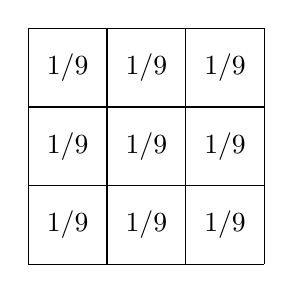
\begin{tikzpicture}
            \draw (0,0) grid (3,3);
            \foreach \u \v in {0.5/0.5,1.5/0.5,2.5/0.5,0.5/1.5,1.5/1.5,2.5/1.5,0.5/2.5,1.5/2.5,2.5/2.5}
            \node at (\u,\v) {\(1/9\)};
        \end{tikzpicture}
        \subcaption{平滑化フィルタ}
        \label{fig:平滑化フィルタ}
    \end{minipage}
    \begin{minipage}[b]{.24\textwidth}
        \centering
        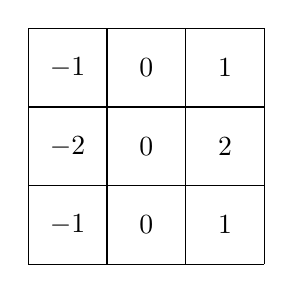
\begin{tikzpicture}
            \draw (0,0) grid (3,3);
            \foreach \u \v \w in {0.5/0.5/{\(-1\)},1.5/0.5/{\(0\)},2.5/0.5/{\(1\)},0.5/1.5/{\(-2\)},1.5/1.5/{\(0\)},2.5/1.5/{\(2\)},0.5/2.5/{\(-1\)},1.5/2.5/{\(0\)},2.5/2.5/{\(1\)}}
            \node at (\u,\v) {\w};
        \end{tikzpicture}
        \subcaption{Prewittフィルタ:横方向}
        \label{fig:Prewittフィルタ_横方向}
    \end{minipage}
    \begin{minipage}[b]{.24\textwidth}
        \centering
        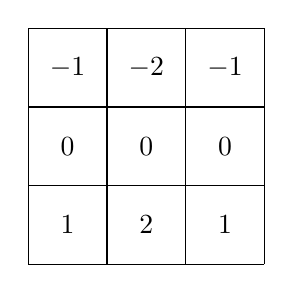
\begin{tikzpicture}
            \draw (0,0) grid (3,3);
            \foreach \u \v \w in {0.5/0.5/{\(1\)},1.5/0.5/{\(2\)},2.5/0.5/{\(1\)},0.5/1.5/{\(0\)},1.5/1.5/{\(0\)},2.5/1.5/{\(0\)},0.5/2.5/{\(-1\)},1.5/2.5/{\(-2\)},2.5/2.5/{\(-1\)}}
            \node at (\u,\v) {\w};
        \end{tikzpicture}
        \subcaption{Prewittフィルタ:縦方向}
        \label{fig:Prewittフィルタ_縦方向}
    \end{minipage}
    \begin{minipage}[b]{.24\textwidth}
        \centering
        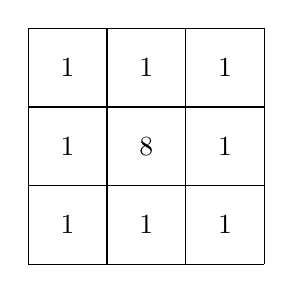
\begin{tikzpicture}
            \draw (0,0) grid (3,3);
            \foreach \u \v in {0.5/0.5,1.5/0.5,2.5/0.5,0.5/1.5,2.5/1.5,0.5/2.5,1.5/2.5,2.5/2.5}
            \node at (\u,\v) {\(1\)};
            \node at (1.5,1.5) {\(8\)};
        \end{tikzpicture}
        \subcaption{Laplacianフィルタ}
        \label{fig:Laplacianフィルタ}
    \end{minipage}
    \caption{\(3\times 3\)画像フィルタ}
\end{figure}
\paragraph{色空間変換}この実験では,RGB色空間から,HSV色空間へ変換する.RGB色空間は,赤(Red),緑(Green),青(Blue)の3チャネルで構成する.HSVは色相(Hue),彩度(Saturation),明度(Value)の3チャネルで構成する.
色相は,カラー ホイール上の色の位置に対応する,\(0\)から\(100\)の値,色相の量または中間からの逸脱.特定の色の赤,緑,青成分の中での最大値.いずれも\texttt{double}型で保存される\cite{rgb2hsv}.
HSV色空間の特徴として,人間が色を知覚する方法と類似しており,視覚障害者向けのアクセシビリティ向上に役立つことが挙げられる.たとえば,HSVの「明度」を調節することで,文字が見やすくなる\cite[p.97\ -\ p.98]{画像処理}.
また,人間が色を知覚する方法と類似していることを踏まえて,HSV色空間を用いることで,画像の特徴を抽出しやすくなる.
今回の実験では,自分の手の写真をRGB色空間からHSV色空間へ変換し,肌色領域を抽出する.抽出した肌色領域を白色,そのほかの部分を黒色にして出力する.出力した画像と,RGB色空間における肌色領域を抽出した場合の精度について考察する.